% Author: Dr. Matthias Jung, DL9MJ
% Year: 2020
% TB701

\usepackage{tikz,pgfplots}
\usetikzlibrary{arrows}

\usepackage{amsmath}
\usepackage{unicode-math}
\setmathfont{Fira Math}
\setmathfont[range=up]{Roboto}
\setmathfont[range=it]{Roboto-Italic}
\setmathfont[range=\int]{Fira Math}
\usepackage[euler]{textgreek}

\begin{document}

\pgfplotsset{
  every axis plot/.append style={line width=0.8pt},
}

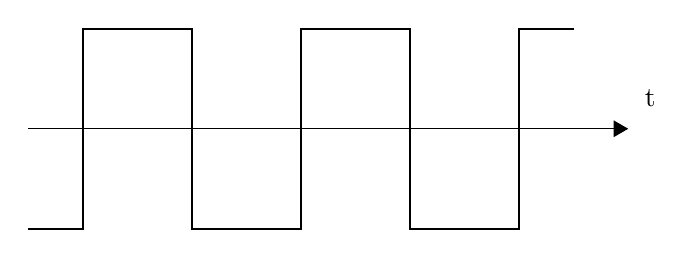
\begin{tikzpicture}
    %\draw (-0.3,4.5) node[]{U};
    \draw ( 7.9, 2.30) node[]{t};
    \begin{axis}[%
        /pgf/number format/1000 sep={ },
        /pgf/number format/use comma,        
        axis lines=middle,
        axis line style={-triangle 60},
        width=3in,
        height=1.5in,
        scale only axis,
        ytick={-1,0,1},
        axis y line=none,
        every major tick/.append style={thick, black},
        grid=major,
        grid style={line width=.1pt, draw=gray!10},
        major grid style={line width=.2pt,draw=gray!50},
        xticklabel=\empty,
        yticklabel=\empty,
        ticks=none,
        xtick style={draw=none},
        ytick style={draw=none},
        xmin=0,
        xmax=5.5,
        ymin=-1.5,
        ymax=1.5,
        xmajorgrids=false,
        ymajorgrids=false,
        tick label style={font=\footnotesize}
    ]
    \addplot+[thick,mark=none,const plot, black]
coordinates
        {(0.0,-1) (0.5,1) (1.5,-1) (2.5,1) (3.5,-1) (4.5,1) (5.0,1)};
\end{axis}
\end{tikzpicture}%
\end{document}
